\chapter{Uhlenbeck compactification as a Bridgeland moduli space}\label{chapter:uhlenbeck}


%%%%%%%%%%%%%%%%%%%%%%%%%%%%%%%%%%%%%%%%%%%%%
%%%%%%%%%%%%%%  INTRODUCTION  %%%%%%%%%%%%%%%
%%%%%%%%%%%%%%%%%%%%%%%%%%%%%%%%%%%%%%%%%%%%%


%%%%%%%%%%%%%%%%%%%%%%%%%%%%%%%%%%%%%%%%%%%%%
%%%%%%%%%%  BRIDGELAND STABILITY %%%%%%%%%%%%
%%%%%%%%%%%%%%%%%%%%%%%%%%%%%%%%%%%%%%%%%%%%%

\section{Bridgeland stability}
In this section we recall definitions and basic notions concerning Bridgeland stability. An excellent exposition of the material is \cite{MS}. 

Let $X$ be a smooth, projective variety, and let $\Kn(X)$ denote its numerical Grothendieck group, that is, the quotient of $K(X)$ by the kernel of the Euler pairing $\chi(-,-)$. A \textbf{(numerical) stability condition} on $X$ is a pair $\si = (\sA, Z)$, where \begin{itemize}
    \item $\sA \subs D^b(X)$ is the heart of a bounded t-structure, and
    \item $Z: \Kn(X) \to \C$ is a {\bf stability function} on $\sA$, that is, a group homomorphism such that for every nonzero object $A \in \sA$, we have 
    \[ Z(A) \in \Hb = \Hh \cup \R_{<0} = \{ r e^{i\pi\phi} \in \C \;|\; r > 0, \; 0 < \phi \le 1 \}. \]
\end{itemize} 
This lets us define a notion of stability in the abelian category $\sA$: we say $A \in \sA$ is \textbf{stable} (resp. \textbf{semistable}) if for every proper nonzero subobject $A' \subs A$, we have
\[ \nu_Z(A') < \nu_Z(A) \qquad (\mathrm{resp.} \quad \nu_Z(A') \leq \nu_Z(A)), \]
where 
\[ \nu_Z(A) = \begin{cases} -\frac{\re Z(A)}{\im Z(A)} & \mathrm{if} \quad \im Z(A) > 0 \\ +\infty & \mathrm{if} \quad \im Z(A) = 0. \end{cases} \]
With this notion of stability, the pair $\si = (\sA, Z)$ must satisfy the following conditions:
\begin{enumerate}[(i)]
    \item Every nonzero $A \in \sA$ has a {\bf Harder-Narasimhan filtration}
    \[ 0 = A_0 \subsetneq A_1 \subsetneq \cdots \subsetneq A_{m-1} \subsetneq A_m = A, \]
    where each quotient $F_i = A_i/A_{i-1}$ is semistable and
    \[ \nu_Z(F_1) > \cdots > \nu_Z(F_m).  \]
    \item {\bf Support property}: there is a symmetric bilinear form $Q$ on $\Kn(X) \otimes \R$ that is negative definite on the kernel of $Z$, and $Q(A, A) \ge 0$ for every semistable object $A \in \sA$.
\end{enumerate}

The set $\Stab(X)$ of stability conditions on $X$ has a natural topology with respect to which the map 
\[ \Stab(X) \to \Hom(\Kn(X), \C), \quad (\sA, Z) \mapsto Z \]
is a local homeomorphism. Moreover, for a given numerical class $v \in \Kn(X)$ there is a locally finite collection of real codimension 1 walls inside $\Stab(X)$ such that the sets of stable and semistable objects remains constant when $\si$ varies within a connected component of the complement of the walls. 

If $C$ is a curve, an example of a stability condition on $C$ is given by $\si = (\Coh(C), Z)$ with $Z(E) = -\deg(E) + i \rk(E)$, giving rise to the classical slope-stability. However, if $\dim X \ge 2$, the standard heart $\Coh(X) \subs D^b(X)$ can never be the heart of a stability condition, see \cite[Lemma 2.7]{toda-limitstable}. 

%%%%%%%%%%%%%%%%%%%%%%%%%%%%%%%%%%%%%%%%

\subsection{Stability conditions on surfaces}\label{section:stabcondsurf}
We now recall a construction of stability conditions on the derived category of a smooth, projective surface $X$ equipped with a very ample divisor $H$. This is achieved by tilting the standard heart $\Coh(X) \subs D^b(X)$ with respect to $\mu$-stability. 

Fix a real divisor class $B \in N^1(X)_\R$. The {\bf $B$-twisted Chern character} is defined by
\[ \ch^B = e^{-B}\cdot \ch, \]
with graded pieces
\[ \ch^B_0 = \ch_0 = \rk, \quad \ch^B_1 = \ch_1 - B \cdot \ch_0, \quad \ch^B_2 = \ch_2 - B \cdot \ch_1 + \frac{B^2}{2} \ch_0. \]
Define the {\bf $B$-twisted slope function} on $\Coh(X)$ by
\[ \mu_B(E) = \frac{H \cdot \ch^B_1(E)}{H^2 \cdot \ch^B_0(E)} = \frac{H \cdot \ch_1(E)}{H^2 \cdot \ch_0(E)} - \frac{H \cdot B}{H^2} \]
if $\rk(E) > 0$, and $\mu_B(E) = \infty$ if $\rk(E) = 0$, i.e. $E$ is a torsion sheaf. Note that this differs from the usual slope function $\mu$ only by the additive constant $-H\cdot B/H^2$ and hence defines the same notion of stability on $\Coh(X)$. 

Since Harder-Narasimhan filtrations into $\mu$-semistable factors exist, for every real number $\be$ we obtain a torsion pair on $\Coh(X)$ by setting
\begin{align*}
    \sT_\be & = \{ E \in \Coh(X) \;|\; \mu_B(F) > \be \mathrm{\;for\;every\;semistable\;factor\;} F \mathrm{\;of\;} E \}, \\
    \sF_\be & = \{ E \in \Coh(X) \;|\; \mu_B(F) \le \be \mathrm{\;for\;every\;semistable\;factor\;} F \mathrm{\;of\;} E \}.
\end{align*}
Thus, we obtain a heart $\Coh^\be(X) = \langle \sF_\be[1], \sT_\be \rangle \subs D^b(X)$ as the full subcategory whose objects are precisely those $E \in D^b(X)$ fitting in an exact triangle
\[ F[1] \to E \to T, \]
where $F \in \sF_\be, T \in \sT_\be$. 

For any $\al \in \R_{>0}$ we define a map $Z_{\al,\be}: \Kn(X) \to \C$ by setting
\begin{align*}
    Z_{\al, \be}(E) & = -\int_X e^{-(\be + i \al)H} \ch^B(E) \\
    & = \frac{\al^2 - \be^2}{2} H^2 \ch^B_0(E) + \be H\cdot\ch^B_1(E) - \ch^B_2(E) \\
    & \quad  + i\al(H \cdot \ch^B_1(E) - \be H^2 \ch^B_0(E)).
\end{align*}
We denote the associated slope function on $\Coh^\be(X)$ by $\nu_{\al,\be}$. It is shown in \cite{bridgelandK3} and \cite{ABL13} that the pair $\si_{\al,\be} = (\Coh^\be(X), Z_{\al,\be})$ is a stability condition on $X$. 

An object $E \in \Coh^\be(X)$ is called \textbf{polystable} with respect to $\si_{\al,\be}$ if 
\[ E \cong \bigoplus_i E_i \] 
where $E_i \in \Coh^\be(X)$ is $\si_{\al,\be}$-stable and $\nu_{\al,\be}(E_i) = \nu_{\al,\be}(E)$ for each $i$. Every $\si_{\al,\be}$-semistable object $E \in \Coh^\be(X)$ has a \textbf{Jordan-H\"older filtration}
\[ 0 = E_0 \subsetneq E_1 \subsetneq \ldots \subsetneq E_{m-1} \subsetneq E_m = E \]
where the successive quotients $E_i/E_{i-1}$ are $\si_{\al,\be}$-stable with 
\[ \nu_{\al,\be}(E_i/E_{i-1}) = \nu_{\al,\be}(E) \] 
for $i = 1,\ldots,m$. The \textbf{associated graded object} of $E$ is the direct sum 
\[ \gr(E) = \bigoplus_i E_i/E_{i-1}, \] 
unique up to noncanonical isomorphism, and two semistable objects $E$ and $E'$ are \textbf{S-equivalent} if $\gr(E) \cong \gr(E')$.

We will need the following observation. 
\begin{lem}\label{ss-ses}
    If $E \in \Coh^\be(X)$ and $\im Z_{\al,\be}(E) = 0$, then in the above triangle 
    \[ F[1] \to E \to T, \]
    $T$ has 0-dimensional support, and $F$ is a $\mu$-semistable sheaf with $\mu_B(F) \\ = \be$.
\end{lem}
\begin{proof}
    Note that for a coherent sheaf $G$, we have $\im Z_{\al,\be}(G) > 0$ (resp. $= 0$) if and only if $\mu_B(G) > \be$ (resp. $= \be$). It follows from the construction that for any $E \in \Coh^\be(X)$,
    \[ \im Z_{\al,\be}(E) = \im Z_{\al,\be}(T) - \im Z_{\al,\be}(F) \]
    and $\im Z_{\al,\be}(T), -\im Z_{\al,\be}(F) \ge 0$. 
    
    First, if $T$ has positive rank, then by assumption $\mu_B(T) > \be$, and so $\im Z_{\al,\be}(E) > 0$. Hence $T$ must have rank 0. If the support of $T$ is 1-dimensional, then \[ \im Z_{\al,\be}(T) = \al H \cdot \ch^B_1(E) = \al H \cdot \ch_1(E) > 0 \]
    since $H$ is ample. This means that $T$ must have 0-dimensional support.
    
    Second, if $F$ is not $\mu$-semistable, then it has a Harder-Narasimhan filtration
    \[ 0 \neq F_1 \subset F_2 \subset \cdots \subset F_{m-1} \subset F_m = F \]
    with respect to $\mu$ with $m \ge 2$, and 
    \[ \im Z_{\al,\be}(F_i/F_{i-1}) \le 0 \quad \mathrm{for\;all}\; i, \quad \mathrm{and} \quad \im Z_{\al,\be}(F_m/F_{m-1}) < 0. \] 
    But then
    \[ - \im Z_{\al,\be}(F) = - \sum_{i=1}^m \im Z_{\al,\be}(F_i/F_{i-1}) > 0. \]
    Thus, $F$ must be $\mu$-semistable.
\end{proof}

\iffalse
We recall why $Z_{\al,\be}$ is a stability function on $\Coh^\be(X)$. That $\im Z_{\al,\be}(E) \ge 0$ for $E \in \Coh^\be(X)$ follows from the construction of the heart $\Coh^\be(X)$. If in the above triangle $T \in \sT_\be$ has 1-dimensional support, then $\ch^B_0(T) = 0$ while $H \cdot \ch^B_1(T) = H \cdot \ch_1(T) > 0$ and in particular $\im Z_{\al,\be}(E) > 0$. Thus, if $\im Z_{\al,\be}(E) = 0$, we have a triangle 
\[ F[1] \to E \to T, \]
where $T$ has 0-dimensional support, and $F$ is a $\mu$-semistable sheaf with $\mu_B(F) = \be$. To verify that $\re Z_{\al,\be}(E) < 0$, we write
\begin{align*} 
    -\re Z_{\al,\be}(E) & = \ch^B_2(T) + \frac{\al^2 - \be^2}{2} H^2 \ch^B_0(F) + \be H\cdot\ch^B_1(F) - \ch^B_2(F) \\
    & = \ch^B_2(T) + \frac{\al^2}{2} H^2 \ch^B_0(F) - \frac{1}{2}\left(\frac{H\cdot \ch^B_1(F)}{H^2 \ch^B_0(F)}\right)^2 H^2 \ch^B_0(F) \\
    & \;\; + \frac{H \cdot \ch^B_1(F)}{H^2 \ch^B_0(F)} H \cdot \ch^B_1(F) - \ch^B_2(F) \\
    & = \ch^B_2(T) + \frac{\al^2}{2} H^2 \ch^B_0(F) + \frac{(H\cdot \ch^B_1(F))^2}{2 H^2 \ch^B_0(F)} - \ch^B_2(F).
\end{align*}
Now $\ch^B_2(T) = \ch_2(T) \ge 0$ since $T$ has 0-dimensional support, and $\frac{\al^2}{2}H^2 \ch^B_0(F) > 0$ since $\ch^B_0(F) = \rk F > 0$. Thus, we must show that
\begin{equation}\label{bogomolovB}
    (H \cdot \ch^B_1(F))^2 - 2 H^2 \ch^B_0(F) \ch^B_2(F) \ge 0.
\end{equation} 
For this, since $H$ is ample, a consequence of the Hodge index theorem is that
\[ H^2 \ch^B_1(F)^2 \le (H \cdot \ch^B_1(F))^2, \]
and so
\begin{align*}
    (H \cdot \ch^B_1(F))^2 - 2 H^2 \ch^B_0(F) \ch^B_2(F) & \ge H^2 \ch^B_1(F)^2 - 2 H^2 \ch^B_0(F) \ch^B_2(F) \\
    & = H^2 (\ch^B_1(F)^2 - 2 \ch^B_0(F) \ch^B_2(F)) \\
    & = H^2 (\ch_1(F)^2 - 2 \ch_0(F) \ch_2(F)),
\end{align*}
where the last line is a direct computation. But $H^2 > 0$ since $H$ is ample, and since $F$ is $\mu$-semistable, the Bogomolov inequality states 
\[ \ch_1(F)^2 - 2 \ch_0(F) \ch_2(F) \ge 0. \]
\fi

\subsection{Wall-and-chamber structure}\label{subsection:wallandchamber}
We visualize the stability conditions $\si_{\al,\be} = (\Coh^\be(X), Z_{\al,\be})$ as living in the upper half-plane with horizontal $\be$-axis and vertical $\al$-axis. The wall-and-chamber structure in the $(\al,\be)$-plane was analyzed in \cite{maciocia} and turns out to be rather simple. If $v \in \Kn(X)$ is a class of positive rank, then there is a unique vertical wall at 
\[ \be_0 = \frac{H \cdot \ch_1^B(v)}{H^2 \ch_0(v)}, \] and on each side of the vertical wall, there is a nested sequence of semicircles with center on the $\be$-axis and contained in a largest semicircle. In particular, on either side of the vertical wall, there is an unbounded open chamber. The walls in the $(\al,\be)$-plane are pairwise disjoint, and so there is no further wall-and-chamber decomposition within each wall. In the unbounded open chamber left of the vertical wall, $\si$-stability coincides with Gieseker stability.
\begin{center}
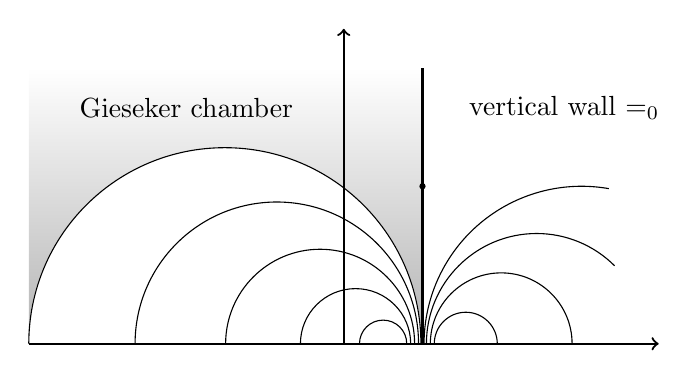
\begin{tikzpicture}

\shadedraw[bottom color=black!30!white,top color=white,draw=white] (-4,0) arc (180:0:2.49) -- (0,0) -- (1,0) -- (1,3.5) -- (-4,3.5);

\draw[thick,->] (-4,0) -- (4,0) node[anchor=south east] {$\be$};
\draw[thick,->] (0,0) -- (0,4) node[anchor=north west] {$\al$};

\draw[thick] (1,0) -- (1,3.5);


\draw[] (0.98,0) arc (0:180:2.49);
\draw[] (0.95,0) arc (0:180:1.8);
\draw[] (0.9,0) arc (0:180:1.2);
\draw[] (0.85,0) arc (0:180:0.7);
\draw[] (0.8,0) arc (0:180:0.3);

\draw[] (1.02,0) arc (180:80:2);
\draw[] (1.05,0) arc (180:45:1.4);
\draw[] (1.1,0) arc (180:0:0.9);
\draw[] (1.15,0) arc (180:0:0.4);

\draw (-2,3) node {Gieseker chamber};
\draw (2.8,3) node {vertical wall $\be = \be_0$};
\fill (1,2) circle (0.04) node[anchor=east] {$\si$};

\end{tikzpicture}
\end{center}
Our goal is to study the moduli space of semistable objects when $\si$ lies on the vertical wall.

\subsection{Stability on the vertical wall}\label{section:stabvertwall}
In this subsection we classify stable and semistable objects on the vertical wall. Let $v \in \Kn(X)$ be a class of positive rank, and let 
\[ (\Coh^{\be_0}(X), Z_{\al,\be_0}) \in \Stab(X) \] 
be the stability condition constructed in the previous section with 
\[ \be_0 = \frac{H \cdot \ch_1^B(v)}{H^2 \ch_0(v)} \quad \mathrm{and} \quad \al > 0. \] Note that since other walls do not intersect the vertical wall, the sets of stable and semistable objects are independent of $\al$.

We first note that there are no nonzero objects in $\Coh^{\be_0}(X)$ with numerical class $v$. Namely, by Lemma \ref{ss-ses}, any object $E \in \Coh^{\be_0}(X)$ with $\im Z_{\al,\be_0}(E) = 0$ fits in a triangle
\[ F[1] \to E \to T, \]
where $T$ has 0-dimensional support and $F$ is $\mu$-semistable. But $\rk(E) = \rk(T) + \rk(F[1]) = -\rk(F) \le 0$, while $\rk(v) > 0$ by assumption. Therefore, it is convenient to instead consider the stability condition 
\[ \si = (\sA, Z), \quad \mathrm{where} \quad \sA = \Coh^{\be_0}(X)[-1], \quad Z = -Z_{\al,\be_0}. \] 
Note that this does not change the slope function $\nu = -\re Z/\im Z$. By definition, the heart $\sA$ consists of objects $E$ with fitting in a triangle
\[ F \to E \to T[-1] \]
where $F \in \sF_{\be_0}, T \in \sT_{\be_0}$.

The next proposition gives a description of stable and semistable objects in $\sA$ of slope $\nu = \infty$ with respect to $\si$. This includes objects of class $v \in \Kn(X)$. Part (i) will be crucial in the proof that the moduli space $M^\si(v)$ of semistable objects of class $v$ is projective, and part (iii) will let us identify $M^\si(v)$ with the Uhlenbeck compactification of the moduli of $\mu$-stable vector bundles, at least on the level of points.
\begin{prop}\label{ss-object-vertical-classification}
    Let 
    \[ \si = (\sA, Z), \quad \mathrm{where} \quad \sA = \Coh^{\be_0}(X)[-1], \quad Z = -Z_{\al,\be_0}. \]
    \begin{enumerate}[(i)]
        \item Any object $E \in \sA$ with $\nu(E) = \infty$ is $\si$-{\bf semistable} and fits in a triangle
        \[ F \to E \to T[-1] \]
        where $T$ is a sheaf supported in dimension 0, and $F$ is a $\mu$-semistable sheaf of slope $\mu_B(F) = \be_0$. 
        \item An object $E \in \sA$ with $\nu(E) = \infty$ is $\si$-{\bf stable} if and only if in the above triangle either $F$ is a $\mu$-stable locally free sheaf and $T = 0$, or $T = \Oh_p$ is the structure sheaf of a closed point $p \in X$ and $F = 0$.
        \item An object $E \in \sA$ of class $v$ is $\si$-{\bf polystable} if and only if
        \[ E \cong \left(\bigoplus_i F_i\right) \oplus \left(\bigoplus_j \Oh_{p_j}[-1]\right), \]
        where each $F_i$ is a $\mu$-stable locally free sheaf of slope $\mu = \mu_B(v)$, and each $p_j \in X$ is a closed point.
    \end{enumerate}
\end{prop}
Part (i) of Proposition \ref{ss-object-vertical-classification} follows from Lemma \ref{ss-ses} and the constructions, while part (iii) follows from part (ii) by the definition of polystability. We prove part (ii)
in a series of lemmas below. Lemmas \ref{muStableLfIsSigmaStable} and \ref{skyscraperIsSigmaStable} show that $\mu$-stable locally free sheaves and shifted skyscraper sheaves are $\si$-stable, and Lemmas \ref{sigmaStablePosRkIsMuStable} and \ref{sigmaStableRk0isSkyscraper} show the converse.
\begin{lem}\label{muStableLfIsSigmaStable}
    A $\mu$-stable locally free sheaf $E$ with $\rk(E) > 0$ and $\mu_B(E) = \be_0$ is $\si$-stable.
\end{lem}
\begin{proof}
    Let $F \hookrightarrow E$ be an inclusion in $\sA$ with $\nu(F) = \infty$. We must show $F = 0$ or $F = E$. The induced short exact sequence
    \[ 0 \to F \to E \to G \to 0 \]
    is by definition an exact triangle in $D^b(X)$ with each vertex in $\sA$. Cohomology with respect to the standard t-structure leads to an exact sequence
    \[ 0 \to \sH^0(F) \to E \to \sH^0(G) \to \sH^1(F) \to 0 \to \sH^1(G) \to 0 \]
    of sheaves. This immediately implies that $\sH^1(G) = 0$, i.e. $G = \sH^0(G)$, and that $\sH^0(F)$ is a subsheaf of $E$.
    
    We have three cases.
    \begin{itemize}
        \item If $\sH^0(F) \xrightarrow{\sim} E$, then $G \xrightarrow{\sim} \sH^1(F)$. But $G \in \sF_{\be_0}, \sH^1(F) \in \sT_{\be_0}$, so we must have $G = \sH^1(F) = 0$, hence $F = \sH^0(F) = E$.
        
        \item If $\sH^0(F)$ is a proper, nonzero subsheaf of $E$, then by the assumption on $E$ we have $\mu_B(\sH^0(F)) < \mu_B(E) = \be_0$. Let $N$ denote the image of the map $E \to G$, so that we have the short exact sequences
        \[ 0 \to \sH^0(F) \to E \to N \to 0 \]
        and 
        \[ 0 \to N \to G \to \sH^1(F) \to 0. \]
        By assumption, $\nu(G) = \infty$ so $G$ is $\mu$-semistable, and thus $\mu_B(N) \le \mu_B(G)$. This gives the absurd inequality 
        \[ \be_0 = \mu_B(E) < \mu_B(N) \le \mu_B(G) \le \mu_B(\sH^1(F)) \le \be_0. \]
        Thus, this case is impossible.
        
        \item If $\sH^0(F) = 0$, then $F = \sH^1(F)[-1]$. Denote $F' = \sH^1(F)$. The short exact sequence
        \[ 0 \to E \to G \to F' \to 0 \]
        implies 
        \[ H\cdot \ch^B_1(G) = H\cdot \ch^B_1(E) + H\cdot \ch^B_1(F'). \]
        Assume for contradiction that $\rk(F') > 0$. Since $\rk(G) \ge \rk(E) > 0$ by assumption, from the above equality and the definition of $\mu_B$ we obtain
        \begin{align*} \be_0 \rk(E) + \mu_B(F') \rk(F') & = \mu_B(E) \rk(E) + \mu_B(F') \rk(F') \\
        & = \mu_B(G) \rk(G) \\
        & \le \be_0 \rk(G), \end{align*}
        so that
        \[ \mu_B(F') \rk(F') \le \be_0(\rk(G) -  \rk(E)) = \be_0 \rk(F'). \]
        However, since $\mu_B(F') > \be_0$, this inequality is impossible. Thus, $\rk(F') = 0$, which also implies $\rk(E) = \rk(G)$ and $\ch^B_1(F') = \ch_1(F')$. 
        
        Next, assume for contradiction that $F'$ has 1-dimensional support. Since $H$ is ample, this implies $H \cdot \ch^B_1(F') > 0$. But on the other hand, 
        \[ \mu_B(G) H^2 \rk(G) = \mu_B(E) H^2 \rk(E) + H \cdot \ch^B_1(F'), \]
        so that
        \[ H \cdot \ch^B_1(F') = H^2 (\mu_B(G) - \be_0)\rk(E) \le 0 \]
        since by assumption $\mu_B(G) \le \be_0$, again a contradiction. Thus, $F'$ has 0-dimensional support. Now if $F' \neq 0$, then we have a locally free subsheaf $E$ of a torsion-free sheaf $G$ with 0-di\-men\-sion\-al quotient $F'$. But as mentioned in \cite[Example 1.1.16]{HL}, the quotient $G/E$ has no 0-dimensional associated points. Thus, we must have $F' = 0$.
    \end{itemize} 
\end{proof}

\begin{lem}\label{skyscraperIsSigmaStable}
    The shifted skyscraper sheaf $\Oh_p[-1]$ is $\si$-stable for every closed point $p \in X$.
\end{lem}
\begin{proof}
    Let $F \hookrightarrow \Oh_p[-1]$ be an inclusion in $\sA$ with $\nu(F) = \infty$. We must show $F = 0$ or $F = \Oh_p[-1]$. Like above, the induced short exact sequence
    \[ 0 \to F \to \Oh_p[-1] \to G \to 0 \]
    in $\sA$ yields the exact sequence
    \[ 0 \to \sH^0(G) \to F \to \Oh_p \to \sH^1(G) \to 0 \]
    of sheaves, and $F = \sH^1(F)$. If $\Oh_p \xrightarrow{\sim} \sH^1(G)$, then $\sH^0(G) \cong F$, and since $\sH^0(G) \in \sF_\be, F \in \sT_\be$, we have $F = 0$.
    
    If on the other hand $\sH^1(G) = 0$, then $G = \sH^0(G)$, and the short exact sequence
    \[ 0 \to G \to F \to \Oh_p \to 0 \]
    implies that $\mu_B(G) = \mu_B(F)$, and we once again see that $G = F = 0$, a contradiction.
\end{proof}

%mmmmmme....................rrrrrrrrrrrrrrrr        <------ Fennel, July 8, 2020. (Fennel is a two-month old kitten.)

\begin{lem}\label{sigmaStablePosRkIsMuStable}
    If $E \in \sA$ is a $\si$-stable object with $\rk(E) > 0$ and $\nu(E) = \infty$, then $E$ is a $\mu$-stable locally free sheaf.
\end{lem}
\begin{proof}
    The object $E$ fits in an exact triangle
    \[ F \to E \to T[-1] \]
    where $F$ is a $\mu$-semistable torsion-free sheaf with $\mu_B(F) = \be_0$ and $T$ is a 0-dimensional sheaf. If $T \neq 0$, then $F$ is a destabilizing subobject of $E$ in $\sA$ unless $F = 0$, in which case $\rk(E) = -\rk(T) = 0$, contrary to the assumption. Thus, $T = 0$ and $E$ is a $\mu$-semistable sheaf.
    
    We next show that $E$ is locally free. Since $E$ is torsion-free, the canonical evaluation map $E \to E^{\vee \vee}$ is injective with cokernel $Q$ supported in dimension 0. Now $E^{\vee\vee}$ and $Q[-1]$ both lie in the heart $\sA$, so the short exact sequence 
    \[ 0 \to E \to E^{\vee \vee} \to Q \to 0 \]
    of coherent sheaves gives an exact sequence
    \[ 0 \to Q[-1] \to E \to E^{\vee \vee} \to 0 \]
    in $\sA$. Since $\nu(Q[-1]) = \nu(E) = \infty$ and $E$ is stable, we must have $Q = 0$, and so $E \cong E^{\vee\vee}$ is locally free.
    
    To show that $E$ is $\mu$-stable, let
    \[ 0 \subset E_1 \subset \cdots \subset E_r = E \]
    be a Jordan-H\"older filtration into $\mu$-stable factors. If $r > 1$, then $E/E_1$ is a $\mu$-semistable sheaf with $\mu_B(E/E_1) = \be_0$, so the short exact sequence of sheaves
    \[ 0 \to E_1 \to E \to E/E_1 \to 0 \]
    is also a short exact sequence in $\sA$ of objects with $\nu = \infty$, which contradicts the $\si$-stability of $E$. Thus, $E = E_1$ is $\mu$-stable.
\end{proof}

\begin{lem}\label{sigmaStableRk0isSkyscraper}
    If $E \in \sA$ is $\si$-stable with $\rk(E) = 0$ and $\nu(E) = \infty$, then $E = \Oh_p[-1]$ for some closed point $p \in X$.
\end{lem}
\begin{proof}
    From the triangle
    \[ F \to E \to T[-1] \]
    as above, we get 
    \[ 0 = \rk(E) = \rk(F) - \rk(T) = \rk(F), \]
    so since $F$ is torsion-free, we must have $F = 0$, and $E = T[-1]$ is the shift of a 0-dimensional sheaf. But any proper subsheaf $T' \subs T$ is also 0-dimensional, so $T'[-1] \in \sA$ is a destabilizing subobject of $E$ with respect to $\si$. Thus, $T$ must have length 1, and so $T = \Oh_p$ for some $p \in X$.
\end{proof}

\begin{rmk}
Proposition \ref{ss-object-vertical-classification} can also be deduced from \cite[Proposition 2.2]{huy} as follows. Any stable object $E \in \sA$ is minimal, since a nonzero surjection $E \twoheadrightarrow E'$ in $\sA$ implies $\nu(E') > \nu(E)$ unless $E' = E$. Conversely any minimal object is automatically stable. Although \cite[Proposition 2.2]{huy} is stated in the case when $X$ is a K3 surface, the proof works for any surface.
\end{rmk}

%%%%%%%%%%%%%%%%%%%%%%%%%%%%%%%%%%%%%%%%%%%%%
%%%%%%  MODULI OF SEMISTABLE OBJECTS  %%%%%%%
%%%%%%%%%%%%%%%%%%%%%%%%%%%%%%%%%%%%%%%%%%%%%

\section{Moduli of semistable objects}\label{section:moduliofbridgeland}
In this section we overview some definitions and results regarding moduli spaces of Bridgeland semistable objects. 

\subsection{Moduli stacks}
Let $X$ be a smooth, projective surface over $\C$ with a very ample divisor $H$, let $v \in \Kn(X)$ be a numerical class, and let $\si = (\sA, Z) \in \Stab(X)$ be a Bridgeland stability condition on $X$. Define a category fibered in groupoids $\sM^\si(v)$ over the big \'etale site of $\C$-schemes as follows. The objects of $\sM^\si(v)$ are pairs $(S, \sE)$, where $S$ is a scheme over $\C$, and $\sE \in D^b(S \times X)$ is a complex of coherent sheaves relatively perfect over $S$, and whenever $S$ is of finite type over $\C$, for every closed point $s \in S$, the derived restriction of $E$ to the fiber $\{s\} \times X \cong X$ lies in $\sA$, is $\si$-semistable, and has numerical class $v$. A morphism $(S', \sE') \to (S, \sE)$ in $\sM^\si(v)$ is a pair $(f, f^\sharp)$, where $f: S' \to S$ is a morphism of $\C$-schemes, and $f^\sharp: \sE \to f_* \sE'$ is a morphism in $D^b(S \times X)$ whose adjoint is an isomorphism $f^* \sE \xrightarrow{\sim} \sE'$ in $D^b(S' \times X)$.

If $\si$ is obtained by tilting with respect to $\mu$-stability as in Section \ref{section:stabcondsurf}, then based on work in \cite{lie06}, \cite{ABL13}, and \cite{AP06}, it is proved in \cite{toda08} that $\sM^\si(v)$ is an algebraic stack of finite type over $\C$. 

\subsection{Good moduli spaces}
Recall that if $\sM$ is an algebraic stack, a quasi-compact, quasi-separated morphism $\pi: \sM \to M$ to an algebraic space $M$ is called a {\bf good moduli space}, if the pushforward functor $\pi_*: \Qcoh(\sM) \to \Qcoh(M)$ is exact, and the natural map $\Oh_M \to \pi_*\Oh_\sM$ is an isomorphism.

In \cite{AHLH}, the authors give necessary and sufficient conditions for the existence of a good moduli space in terms of certain valuative criteria. As an application, the authors construct proper good moduli spaces for various moduli stacks $\sM^{\mathrm{ss}}_\sA$ parameterizing objects in an abelian category $\sA$ that are semistable with respect to a rather general notion of stability on $\sA$. This construction includes stacks of Bridgeland semistable objects on a smooth, projective variety $X$ with respect to a numerical stability condition $\si = (\sA, Z) \in \Stab(X)$ whose heart $\sA$ is noetherian and satisfies the ``generic flatness property'', and for which the moduli stacks $\sM^\si(v)$ are of finite type. See \cite[Section 7]{AHLH} for details, especially Theorem 7.25 and Example 7.27. In particular, we have the following.
\begin{thm}\label{gmsexists}
    Let $X$ be a smooth, projective surface over $\C$, let $v \in \Kn(X)$ be a numerical class, and let $\si \in \Stab(X)$ be a stability condition constructed by tilting with respect to slope-stability as in Section \ref{section:stabcondsurf}. The moduli stack $\sM^\si(v)$ of $\si$-semistable objects of class $v$ admits a good moduli space map $\sM^\si(v) \to M^\si(v)$, where $M^\si(v)$ is a proper algebraic space over $\C$. The closed points of $M^\si(v)$ are in bijection with S-equivalence classes of $\si$-semistable objects of class $v$.
\end{thm}



%%%%%%%%%%%%%%%%%%%%%%%%%%%%%%%%%%%%%%%%%%%%%
%%%%%%%%%%%%%  NEF LINE BUNDLE  %%%%%%%%%%%%%
%%%%%%%%%%%%%%%%%%%%%%%%%%%%%%%%%%%%%%%%%%%%%

\section{The nef line bundle}
In \cite{BM}, the authors construct a natural numerical class of line bundles with strong positivity properties on a Bridgeland moduli space $\sM^\si(v)$ that varies with the stability condition $\si$. We recall here the construction and basic properties of the line bundle, as well as identify the line bundle on the vertical wall.

\subsection{Definition and positivity properties}\label{positiveLBdefandprops}
Let $(X,H)$ be a smooth, projective, polarized surface, let $\si = (\sA, Z) \in \Stab(X)$ be a stability condition, and let $v \in \Kn(X)$ be a numerical class. Assume that the moduli stack $\sM^\si(v)$ of $\si$-semistable objects in $\sA$ of class $v$ is algebraic, and denote by $\sE$ the universal complex on $\sM^\si(v) \times X$. Consider the following diagram:
\begin{center}
    \begin{tikzpicture}
    \matrix (m) [matrix of math nodes, row sep=1.5em, column sep=1em]
    { & \sM^\si(v) \times X & \\
    \sM^\si(v) & & X \\};
    \path[->] 
    (m-1-2) edge node[auto,swap] {$ p $} (m-2-1)
    (m-1-2) edge node[auto] {$ q $} (m-2-3)
    ;
    \end{tikzpicture}
\end{center}
The Donaldson morphism
\[ \la_\sE: K_0(X) \to \Pic(\sM^\si(v)), \quad [F] \mapsto \det R p_*(\sE \otimes q^* F) \]
from Section \ref{section:determinantal} induces a map 
\[ \la_\sE: \Kn(X)_\R \to \Num(\sM^\si(v))_\R. \]
Define a real divisor class on $\sM^\si(v)$ by applying the Donaldson morphism to the unique class $w_Z \in \Kn(X)_\R$ determined by the condition
\[ \chi(w_Z, -) = \im\left(-\frac{Z(-)}{Z(v)}\right). \]
This condition indeed defines a unique class since the Euler pairing $\chi(-,-)$ induces a perfect pairing on $\Kn(X)_\R$. Denote this numerical class by $\sL_\si \coloneqq \la_\sE(w_Z)$. The following is \cite[Lemma 3.3]{BM}, and it is the main result of the paper.
\begin{thm}\label{BMpositivity}
    Let $C$ be a projective, integral curve over $\C$, and let $f: C \to \sM^\si(v)$ be a morphism.
    \begin{enumerate}[(1)]
        \item $\deg f^* \sL_\si \ge 0$.
        \item If $\deg f^* \sL_\si = 0$, then for any two closed points $s, t \in C$, the objects \\ $(f \times \id_X)^*\sE|_{\{s\} \times X}$ and $(f\times \id_X)^*\sE|_{\{t\} \times X}$ are S-equivalent.
    \end{enumerate}
\end{thm}
In \cite{BM}, part (2) is stated so that the objects $(f \times \id_X)^*\sE|_{\{t\} \times X}$ are S-equivalent for points $t$ in some nonempty open subscheme $U \subs C$. We deduce the above statement from Theorem \ref{gmsexists} as follows. If $\sM^\si(v) \to M^\si(v)$ denotes the good moduli space map, then the composition $C \to \sM^\si(v) \to M^\si(v)$ maps the dense open set $U$ to a point, hence must be constant, and so the objects $(f\times \id_X)^*\sE|_{\{t\} \times X}$ are all S-equivalent. 

We would like to know that the real divisor class $\sL_\si$ descends to the good moduli space $M^\si(v)$. In \cite{BM} and \cite{nuer} this is done using a so-called quasi-universal family on the stable locus of the moduli space. However, we can achieve this on all of $M^\si(v)$ as follows.
\begin{lem}\label{nefdescendtogms}
    If $w \in K(X)$ is a class whose image in $\Kn(X)_\R$ is a multiple of $w_Z$, then $\la_\sE(w)$ descends to the good moduli space $M^\si(v)$.
\end{lem} 
\begin{proof}
    Write $w = b w_Z$ in $\Kn(X)_\R$ with $b \in \R$. We check the condition in Proposition \ref{lbtogms}. If $E \cong E_1^{\oplus r_1} \oplus \cdots \oplus E_m^{\oplus r_m}$ is a $\si$-polystable object of class $v$, then for each $i$, the complex number $Z(E_i)$ lies on the same ray as $Z(E)$, so that $Z(E_i)/Z(v)$ is real, and so
    \[ \chi(w, E_i) = b\,\chi(w_Z, E_i) = b\,\im\left(-\frac{Z(E_i)}{Z(v)}\right) = 0. \]
    Thus, $\la_\sE(w)$ descends to a line bundle on the good moduli space.    
\end{proof}
This lets us define a numerical class $L_\si$ on $M^\si(v)$ by setting $L_\si = \frac{1}{b}[\sN]$ where $\pi^*\sN = \la_\sE(w)$ such that $w \in K(X)$ satisfies $w \equiv b w_Z$ in $\Kn(X)$ and $b > 0$. The class $L_\si$ is independent of the choice of $w$. We would like to know that $L_\si$ enjoys the same positivity properties as $\sL_\si$.
\begin{lem}\label{gmsnef}
    Let $C$ be a smooth, projective, integral curve over $\C$, and let $g: C \to M^\si(v)$ be a morphism.
    \begin{enumerate}[(1')]
        \item $\deg g^* L_\si \ge 0$.
        \item If $\deg g^* L_\si = 0$, then $g$ is constant.
    \end{enumerate}
\end{lem}
\begin{proof}
    By Lemma \ref{finitecurveextension}, we can find a commutative diagram
    \begin{center}
    \begin{tikzpicture}
    \matrix (m) [matrix of math nodes, row sep=2em, column sep=2em]
    { C' & \sM^\si(v)  \\
    C & M^\si(v) \\};
    \path[->] 
    (m-1-1) edge node[auto] {$ f $} (m-1-2)
    (m-1-1) edge node[auto,swap] {$ \phi $} (m-2-1)
    (m-1-2) edge node[auto] {$ \pi $} (m-2-2)
    (m-2-1) edge node[auto,swap] {$ g $} (m-2-2)
    ;        
    \end{tikzpicture}
    \end{center}
    where $C'$ is a smooth, projective curve, $\phi$ is a finite morphism, and $\pi$ is the good moduli space map. To prove (1') we note that
    \[ \deg(\phi) \deg g^* L_\si = \deg (g \circ \phi)^* L_\si = \deg(\pi \circ f)^* L_\si = \deg f^*\sL_\si \ge 0, \]
    so since $\deg(\phi) > 0$, we get $\deg g^* L_\si \ge 0$.
    
    To prove (2'), assume that $\deg g^*L_\si = 0$. Then also $f^* \sL_\si = 0$, so by part (2) of Theorem \ref{BMpositivity}, the family parameterized by $C'$ consists of S-equivalent objects, so the composition $\pi \circ f: C' \to M^\si(v)$ maps every closed point of $C'$ to the same point $p_0 \in |M^\si(v)|$, and the same holds for $g: C \to M^\si(v)$, and so the scheme-theoretic image of $g$ is a closed point of $M^\si(v)$.
\end{proof}


\subsection{The nef line bundle on the vertical wall}
We can describe the class $w_Z \in \Kn(X)$ more explicitly in the case of the stability condition 
\[ \si = (\sA, Z) = (\Coh^{\be_0}(X)[-1], -Z_{\al, \be_0}), \quad \mathrm{where} \quad \be_0 = \frac{H \cdot \ch_B^1(v)}{H^2 \ch_B^0}, \; \al > 0, \] that is, when $\si$ lies on the vertical wall for $v$. Recall that $H \subs X$ denotes a fixed very ample divisor. Denote $h = [\Oh_H] \in K(X)$.
\begin{propdef}\label{nefclassonverticalwall}
    Let $(X,H)$ be a smooth, projective, polarized surface, let $v \in \Kn(X)$ be a class of positive rank, and let $\si \in \Stab(X)$ lie on the vertical wall for $v$ as in Section \ref{section:stabvertwall}. Define 
    \[ u = -\chi(v \cdot h^2) h + \chi(v \cdot h) h^2 \in K(X). \]
    We have 
    \[ w_Z = -\frac{\al}{\rk(v) Z(v) \deg X} u. \]
\end{propdef}
Note that $Z(v)$ is a negative real number, so $w_Z$ is indeed a positive multiple of $u$. Thus, $\la_\sE(u)$ enjoys the same positivity properties as $\sL_\si = \la_\sE(w_Z)$.
\begin{proof}
    Fix a closed point $p \in X$, and denote the numerical Todd class of $X$ by
    \[ \td_X = 1 - \frac{1}{2} K_X + \chi(\Oh_X) [p]. \]
    We will use the Hirzebruch-Riemann-Roch formula:
    \[ \chi(a \cdot b) = \int_X \ch(a) \ch(b) \td_X \]
    for $a, b \in \Kn(X)$.
    
    Let $a \in K(X)$ be arbitrary. To compute $\chi(a \cdot u)$, we may replace $u$ with something numerically equivalent. Now $h^2 \equiv \deg(X) [\Oh_p]$ by Bertini, and $v \cdot [\Oh_p] = \rk(v)$, so if we set
    \[ u' = - \rk(v) h + \chi(v \cdot h) [\Oh_p] \]
    we can consider the class $\deg(X) u'$ instead of $u$. Moreover, 
    \[ \ch(\Oh_H) = \ch(\Oh_X) - \ch(\Oh_X(-H)) = H - \frac{1}{2} H^2, \quad \ch(\Oh_p) = [p], \]
    so by Hirzebruch-Riemann-Roch,
    \begin{align*}
        \chi(v \cdot h) & = \int_X (\rk(v) + \ch_1(v))\left(H - \frac{1}{2}H^2\right)\left(1 - \frac{1}{2}K_X\right) \\
        & = \ch_1(v) \cdot H - \frac{\rk(v)}{2} H\cdot(H + K_X),
    \end{align*}
    and hence
    \begin{align*}
        \ch(u') & = -\rk(v) \ch(\Oh_H) + \chi(v \cdot [\Oh_H]) \ch(\Oh_p) \\
        & = -\rk(v)\left(H - \frac{1}{2}H^2\right) + \left(\ch_1(v) \cdot H - \frac{\rk(v)}{2} H(H + K_X)\right)[p] \\
        & = -\rk(v) H + \left(\ch_1(v) \cdot H - \frac{\rk(v)}{2} H \cdot K_X\right)[p]
    \end{align*}
    Since $\ch(u')$ is in $A^{\ge 1}(X)$, we only need to know the $A^{\le 1}(X)$-part of $\ch(a)\td_X$, which is
    \[ \ch(a) \td_X = (\ch_0(a) + \ch_1(a)) (1 - \frac{1}{2} K_X) \equiv \ch_0(a) - \frac{1}{2} \ch_0(a) K_X + \ch_1(a). \]
    Putting everything together, we now calculate
    \begin{align*}
        \chi(a \cdot u') & = \int_X \ch(a) \ch(u') \td_X \\
        & = \int_X \left(\ch_0(a) - \frac{1}{2} \ch_0(a) K_X + \ch_1(a)\right)\cdot  \\
        & \quad\left(-\ch_0(v) H + \ch_1(v) H - \frac{1}{2} \ch_0(v) H \cdot K_X\right) \\
        & = H \cdot (\ch_0(a) \ch_1(v) - \ch_0(v) \ch_1(a)) \\
        & = H \cdot (\ch^B_0(a) \ch^B_1(v) - \ch^B_0(v) \ch^B_1(a))
    \end{align*}
    Thus,
    \[ \chi(a \cdot u) = \deg X \cdot \chi(a \cdot u') = \deg X \cdot H (\ch^B_0(a) \ch^B_1(v) - \ch^B_0(v) \ch^B_1(a)). \]
    
    Next we calculate $\im(-Z(a)/Z(v))$. Recall that since $\si$ is on the vertical wall for $v$, the quantity $Z(v)$ is a negative real number, and so 
    \[ \im\left(-\frac{Z(a)}{Z(v)}\right) = -\frac{1}{Z(v)} \im Z(a). \]
    Now 
    \begin{align*}
        \im Z(a) & = \al(\be_0 H^2 \ch^B_0(a) - H \cdot \ch^B_1(a)) \\
        & = \al \left( \frac{H \cdot \ch^B_1(v)}{H^2 \ch^B_0(v)} H^2 \ch^B_0(a) - H \cdot \ch^B_1(a) \right) \\
        & = \frac{\al}{\ch^B_0(v)} H (\ch^B_0(a) \ch^B_1(v) - \ch^B_0(v) \ch^B_1(u)).
    \end{align*}
    Thus, we see that
    \[ \im\left(-\frac{Z(a)}{Z(v)}\right) = -\frac{\al}{\rk(v) Z(v) \deg X} \chi(a \cdot u). \]
\end{proof}

\begin{rmk}
    The calculation of $w_Z$ as in Proposition \ref{nefclassonverticalwall} appears in \cite{liuwanmin} using a dual version of the Donaldson morphism. See in particular \cite[Theorem 4.13(b)]{liuwanmin}
\end{rmk}



%%%%%%%%%%%%%%%%%%%%%%%%%%%%%%%%%%%%%%%%%%%%%
%  PROJECTIVITY OF THE GOOD MODULI SPACE  %%
%%%%%%%%%%%%%%%%%%%%%%%%%%%%%%%%%%%%%%%%%%%%%
\section{Projectivity of the good moduli space}

Let $(X, H)$ be a smooth, projective, polarized surface over $\C$, let $v \in \Kn(X)$ be a nu\-mer\-i\-cal class with $\rk(v) > 0$, and let $\si$ be a stability condition lying on the vertical wall for $\si$ considered in Section \ref{section:stabvertwall}, that is,
\[ \si = (\sA, Z) = (\Coh^{\be_0}(X)[-1], -Z_{\al, \be_0}), \quad \mathrm{where} \quad \be_0 = \frac{H \cdot \ch_B^1(v)}{H^2 \ch_B^0}, \; \al > 0. \]
Let $\sM^\si(v)$ be the stack of $\si$-semistable objects of class $v$ in $\sA$, and let $\sE$ be the universal complex on $\sM^\si(v) \times X$. In this section we prove that the good moduli space $M^\si(v)$ of the stack $\sM^\si(v)$ is projective. 

Recall from Section \ref{positiveLBdefandprops} that $\sL_\si$ denotes the natural nef line bundle on $\sM^\si(v)$ and $L_\si$ the corresponding line bundle on $M^\si(v)$. We will show that $L_\si$ is ample. Since by Lemma \ref{nefdescendtogms}, $L_\si$ is strictly positive on any proper curve in $M^\si(v)$, it suffices to show that $L_\si$ is semiample, meaning that some tensor power is globally generated. Moreover, since by Proposition \ref{vbtogms}, sections of $\sL_\si$ descend to sections of $L_\si$, it suffices to show that $\sL_\si$ is semiample. To produce sections of $\sL_\si$, we expand on techniques used in \cite{li} for constructing a scheme structure on the Uhlenbeck compactification, and in \cite{seshadri} for constructing moduli spaces of vector bundles on a curve. 

The idea is as follows. First, we explain how to obtain a diagram
\begin{center}
    \begin{tikzpicture}
    \matrix (m) [matrix of math nodes, row sep=3em, column sep=0.5em]
    { & \sM^\si(v) \times X & & \sM^\si(v) \times C & \\
    \sM^\si(v) & & X & & C \\};
    \path[left hook->] 
    (m-1-4) edge node[auto,swap] {$ j $} (m-1-2)
    (m-2-5) edge node[auto] {$ i $} (m-2-3)
    ;
    \path[->]
    (m-1-2) edge node[auto,swap] {$ p $} (m-2-1)
    (m-1-2) edge node[pos=0.9,yshift=10pt] {$ q $} (m-2-3)
    (m-1-4) edge node[pos=0.7,yshift=-8pt] {$ p_C $} (m-2-1)
    (m-1-4) edge node[auto] {$ q_C $} (m-2-5)
    ;        
    \end{tikzpicture}
\end{center}
where $C$ is a smooth curve in the linear system $|a H|$ for $a > 0$, together with a locally free sheaf $G$ on $C$, with the property that the determinantal line bundle
\[ \la_{j^* \sE}(G)^\vee = \det(R p_{C*}(j^*\sE \otimes q_C^*G))^\vee \]
is a positive multiple of $\sL_\si$ on $\sM^\si(v)$. 

Next, by analyzing restrictions of $\si$-semistable objects $E$ to $C$, we apply Lemma \ref{detsection}(a) to show that $\la_{j^* \sE}(G)^\vee$ has a canonical global section $\de_G$ on $\sM^\si(v)$. Moreover, we show that for a given $\C$-point $t \in \sM^\si(v)$, we can choose the curve $C$ and the sheaf $G$ so that the section $\de_G$ is nonvanishing at $t$. To do this, recall from Proposition \ref{ss-object-vertical-classification} that the complex $\sE_t$ on $\{t\} \times X = X$ fits in an exact triangle
\[ F \to \sE_t \to T[-1] \]
in $D^b(X)$, where $F$ is a $\mu$-semistable torsion-free sheaf and $T$ is a torsion sheaf with 0-dimensional support. Using a restriction theorem for $\mu$-stability, we show that we can choose $a \gg 0$ and $C \in |a H|$ so that
\begin{enumerate}[(1)]
    \item $C$ avoids the support of $T$, and
    \item the restriction $\sE_t|_C = F|_C$ to $C$ is slope-semistable.
\end{enumerate}
Using a characterization of semistability on a curve due to Faltings and Seshadri, we find a locally free sheaf $G$ on $C$ with the property that 
\[ H^0(C, F|_C \otimes G) = H^1(C, F|_C \otimes G) = 0, \]
and apply Lemma \ref{detsection}(b) to translate this into the nonvanishing of $\de_G$ at $t$.

Finally, by varying $C$ and $G$, we produce a generating set of sections of some power of $\sL_\si$, or equivalently $L_\si$, and use Theorem \ref{gmsexists} and Lemma \ref{gmsnef} to show that the morphism $M^\si(v) \to \p^N$ induced by the sections is finite. From this we conclude that $M^\si(v)$ is projective.

\subsection{Sheaves on curves and the nef line bundle}
We begin to carry out the plan outlined above. To set up some notation, let $C \subs X$ be a smooth, connected curve in the linear system $|a H|$ for some $a > 0$, and consider the diagram:
\begin{center}
    \begin{tikzpicture}
    \matrix (m) [matrix of math nodes, row sep=3em, column sep=0.5em]
    { & \sM^\si(v) \times X & & \sM^\si(v) \times C & \\
    \sM^\si(v) & & X & & C \\};
    \path[left hook->] 
    (m-1-4) edge node[auto,swap] {$ j $} (m-1-2)
    (m-2-5) edge node[auto] {$ i $} (m-2-3)
    ;
    \path[->]
    (m-1-2) edge node[auto,swap] {$ p $} (m-2-1)
    (m-1-2) edge node[pos=0.9,yshift=10pt] {$ q $} (m-2-3)
    (m-1-4) edge node[pos=0.7,yshift=-8pt] {$ p_C $} (m-2-1)
    (m-1-4) edge node[auto] {$ q_C $} (m-2-5)
    ;        
    \end{tikzpicture}
\end{center}
where $p, q, p_C, q_C$ denote the projections, and $i$ and $j$ are closed embeddings. Let $\sE_C \coloneqq j^*\sE$ be the restriction of $\sE$ to $\sM^\si(v) \times C$, which is perfect relative to $\sM^\si(v)$. We have the Donaldson homomorphisms
\[ \la_\sE: K(X) \to \Pic(\sM^\si(v)), \quad \la_{\sE_C}: K(C) \to \Pic(\sM^\si(v)). \]
In addition, for any $n \in \Z$, we have a map $K(X) \to K(X), w \mapsto w(n)$ induced by the map on locally free sheaves $F \mapsto F(n) = F \otimes \Oh_X(n)$. Similarly we have a map $K(X) \to K(C), w \mapsto w|_C$ induced by $F \mapsto F|_C = i^*F$. We denote $h = [\Oh_H] \in K(X)$ as before.

Recall from Proposition \ref{nefclassonverticalwall} that for the class 
\[ u = -\chi(v \cdot h^2) h + \chi(v \cdot h) h^2 \in K(X), \]
the line bundle $\la_\sE(u)$ on $\sM^\si(v)$ is a positive multiple of the natural nef line bundle $\sL_\si$. We first establish the following.
\begin{propdef}\label{nefpowerfromcurves}
    Given an integer $a > 0$ and a smooth, connected curve $C \in |a H|$, define the class
    \[ w \coloneqq -\chi(v \cdot h \cdot [\Oh_C]) \cdot 1 + \chi(v \cdot [\Oh_C]) \cdot h \in K(X). \]
    We have an isomorphism
    \[ \la_{\sE_C}(w|_C) \cong \la_\sE(u)^{a^2}. \]
    Moreover, the class $-w|_C \in K(C)$ has positive rank, and so can be represented by a locally free sheaf $G$ on $C$.
\end{propdef}

The proof of the following simple lemma as well as part of the proof of Proposition \ref{nefpowerfromcurves} below are essentially included in the proof of \cite[Proposition 8.2.3]{HL}.

\begin{lem}\label{Ktheorylemma}
    If $C \in |a H|$ is a curve and $w' \in K(X)$ is arbitrary, then
    \[ \la_\sE(w' - w'(-a)) = \la_{\sE_C}(w'|_C). \]
\end{lem}
\begin{proof}
    Both sides of the equation are linear in $w'$, so it suffices to consider the class $w' = [F]$ for a locally free sheaf $F$ on $X$. On the one hand, we have
    \begin{align*}
        \la_{\sE_C}(F|_C) & = \det R p_{C*}(\sE_C \otimes q_C^* i^* F) \\
        & = \det R p_* j_*(\sE_C \otimes j^* q^* F) \\
        & = \det R p_* (j_*\sE_C \otimes q^* F). \qquad \mathrm{(projection\;formula)}
    \end{align*}
    On the other hand, pulling back the short exact sequence 
    \[ 0 \to \Oh_X(-a) \to \Oh_X \to j_* \Oh_C \to 0 \]
    along $q$, tensoring with $\sE \otimes q^* F$, and applying $R p_*$ gives the exact triangle
    \[ R p_* (\sE \otimes q^*(F \otimes \Oh_X(-a))) \to R p_* (\sE \otimes q^*F) \to R p_* (j_* \sE_C \otimes q^*F) \]
    in $D^b(\sM^\si(v))$, and so we obtain an isomorphism
    \[ \det R p_* (j_* \sE_C \otimes q^*F) \cong \la_\sE(F) \otimes \la_\sE(F(-a))^\vee = \la_\sE(w - w(-a)). \]
\end{proof}

\begin{proof}[Proof of Proposition \ref{nefpowerfromcurves}]
    By Lemma \ref{Ktheorylemma}, for the first statement it is enough to show that
    \[ w - w(-a) = a^2 u. \]
    Since $[\Oh_X(-1)] = 1 - h \in K(X)$, we have
    \[ [\Oh_X(-a)] = [\Oh_X(-1)]^a = (1 - h)^a = 1 - a h + \binom{a}{2} h^2, \]
    so the short exact sequence
    \[ 0 \to \Oh_X(-a) \to \Oh_X \to \Oh_C \to 0 \]
    gives $[\Oh_C] = 1 - [\Oh_X(-a)] = a h - \binom{a}{2} h^2$. In particular, $h \cdot [\Oh_C] = a h^2$. We now calculate
    \begin{align*}
        w - w(-a) & = w \cdot [\Oh_C] \\
        & = (-\chi(v \cdot h \cdot [\Oh_C]) \cdot 1 + \chi(v \cdot [\Oh_C]) \cdot h) (a h - \binom{a}{2} h^2) \\
        & = - \chi(v \cdot ah^2) (a h - \binom{a}{2} h^2) + \chi\left(v \cdot (a h - \binom{a}{2} h^2)\right) a h^2 \\
        & = a^2 ( - \chi(v \cdot h^2) h + \chi(v \cdot h) h^2) = a^2 u.
    \end{align*}
    For the second claim, we note that 
    \[ -w|_C = \chi(v|_C \cdot h|_C) \cdot 1 - \chi(v|_C) \cdot h|_C = a \rk(v) \deg X \cdot 1 - \chi(v|_C) \cdot h|_C, \]
    and so 
    \[ \rk(w|_C) = a \rk(v) \deg X \rk(1) - \chi(v|_C) \rk(h|_C) = a \rk(v) \deg(X) > 0. \] 
    Since $C$ is smooth, projective, and connected, the natural map 
    \[ K(C) \to \Z \oplus \Pic(C), \quad [F] \mapsto (\rk F, \det F) \] 
    is an isomorphism. Moreover, any class $(m, L) \in \Z \oplus K(C)$ with $m > 0$ can be represented by a locally free sheaf: take for instance $G = \Oh_C^{\oplus m-1} \oplus L$. In particular, there exist locally free sheaves $G$ of class $- w|_C$ on $C$.
\end{proof}

\subsection{Producing sections}
Our next task is to show that the construction of Proposition \ref{nefpowerfromcurves} yields a canonical section $\de_G$ of the line bundle $\la_{\sE_C}(G)^\vee \cong \la_\sE(u)^{m a^2}$ on $\sM^\si(v)$, and that by choosing $C$ and $G$ carefully, this section is nonzero at a given point $t \in \sM^\si(v)$. After some preparations, we prove this in Proposition \ref{globalgen}. In the proof, Lemmas \ref{restsingle} and \ref{hypercohovanishing} will be used to apply Lemma \ref{detsection}(a), and Lemmas \ref{restsemistable} and \ref{seshadrimainlemma1} to apply Lemma \ref{detsection}(b).

\begin{lem}\label{restsingle} 
    Let $X$ be a smooth, projective surface and $C \subs X$ a smooth, projective curve. Assume $E \in D^b(X)$ fits in a triangle
    \[ F \to E \to T[-1], \]
    where $F$ is a torsion-free sheaf and $T$ is a torsion sheaf with 0-di\-men\-sion\-al support. The derived restriction $E|_C^\LL$ fits in a triangle
    \[ \sH^0(E|_C^\LL) \to E|_C^\LL \to \sH^1(E|_C^\LL)[-1] \]
    in $D^b(C)$, where $\sH^1(E|_C^\LL)$ is a torsion sheaf.
\end{lem}
\begin{proof}
Derived restriction to $C$ is a functor of triangulated categories, so we obtain a triangle
\[ F|_C^\LL \to E|_C^\LL \to T|_C^\LL[-1], \]
which yields a long exact sequence of cohomology sheaves
\[ \cdots \to \sH^i(F|_C^\LL) \to \sH^i(E|_C^\LL) \to \sH^i(T|_C^\LL[-1]) \to \sH^{i+1}(F|_C^\LL) \to \cdots. \]
To understand the terms in this sequence, we study the derived restrictions $F|_C^\LL$ and $T|_C^\LL$. Since pushforward of coherent sheaves along the inclusion $C \hookrightarrow X$ is exact, we may as well study the derived tensor products $F \otimes^\LL \Oh_C$ and $T \otimes^\LL \Oh_C$, where $\Oh_C$ is the structure sheaf of $C$ viewed as an $\Oh_X$-module. 

Since $C \subs X$ is a Cartier divisor, $\Oh_C$ has a resolution by line bundles
\[ 0 \to \Oh_X(-C) \xrightarrow{f} \Oh_X \to \Oh_C \to 0. \]
Thus, the objects $F \otimes^\LL \Oh_C$ and $T \otimes^\LL \Oh_C$ are represented by the complexes
\[ \sF = [F(-C) \xrightarrow{f} F] \qquad \mathrm{and} \qquad \sT = [T(-C) \xrightarrow{f} T] \]
respectively, where $F$ and $T$ are placed in degree 0. 


Since $F$ is by assumption torsion-free, the map $f: F(-C) \to F$ is injective. Thus, we see that $\sH^0(F|_C^\LL) = \sH^0(\sF) = F|_C$ agrees with the ordinary restriction, and $\sH^i(F|_C^\LL) = \sH^i(\sF) = 0$ for $i \neq 0$. Moreover, from $\sT$ we see that $\sH^{-1}(T|_C^\LL) = \sH^{-1}(\sT)$ is a subsheaf of $T(-C) \cong T$, and $\sH^0(T|_C^\LL) = \sH^0(\sT)$ is a quotient of $T$, hence both are 0-dimensional, and $\sH^i(T|_C^\LL) = 0$ for $i \neq -1, 0$.

We now return to the triangle
\[ F|_C^\LL \to E|_C^\LL \to T|_C^\LL[-1] \]
at the beginning of the proof. Taking into account the shift in the last term, we obtain an exact sequence of cohomology sheaves
\[ 0 \to F|_C \to \sH^0(E|_C^\LL) \to \sH^{-1}(T|_C^\LL) \to 0 \to \sH^1(E|_C^\LL) \to \sH^0(T|_C^\LL) \to 0, \]
and also see that $\sH^i(E|_C^\LL) = 0$ if $i \neq 0,1$. In particular, $E|_C^\LL$ is supported in degrees $0$ and $1$, and $\sH^1(E|_C^\LL) \cong \sH^0(T|_C^\LL)$ is a torsion sheaf on $C$.
\end{proof}

\begin{lem}\label{hypercohovanishing}
    If $C$ is a projective curve and $E \in D^b(C)$ fits into a triangle
    \[ F \to E \to T[-1], \]
    with $F, T \in \Coh(C)$ and $T$ has 0-dimensional support, then the hypercohomology groups of $E$ satisfy
    \[ \Hh^i(C, E) = 0 \qquad \mathrm{for} \; i \neq 0, 1. \]
\end{lem}
\begin{proof}
    We have a long exact sequence of hypercohomology groups
    \[ \cdots \to \Hh^i(C, F) \to \Hh^i(C, E) \to \Hh^i(C, T[-1]) \to \Hh^{i+1}(C, F) \to \cdots. \]
    Since $\Hh^i(C, F) = 0$ whenever $i \neq 0, 1$, and 
    \[ \Hh^i(C, T[-1]) = \Hh^{i-1}(C, T) = 0 \] 
    whenever $i \neq 1$, the group $\Hh^i(C, E)$ can be nonzero only if $i = 0,1$.
\end{proof}

We pause to recall that $\si = (\sA, Z)$ denotes a stability condition on the vertical wall for the class $v \in \Kn(X)$, and that by Proposition \ref{ss-object-vertical-classification}, any $\si$-semistable object $E \in \sA$ of class $v$ fits in a triangle
\[ F \to E \to T[-1] \]
where $F$ is a $\mu$-semistable torsion-free sheaf and $T$ is a torsion sheaf with 0-dimensional support. 

\begin{lem}\label{restsemistable}
    If $E \in \sA \subs D^b(X)$ is a $\si$-semistable object of class $v$, there exists a smooth, projective, connected curve $C \subs X$ in the linear system $|a H|$ for $a \gg 0$ such that the derived restriction of $E$ to $C$ is a slope-semistable locally free sheaf.    
\end{lem}
\begin{proof} 
We use Flenner's restriction theorem, \cite[Theorem 7.1.1]{HL}. Specialized to the case at hand, it states the following. Let $a$ be an integer satisfying
\[ \frac{\binom{a+2}{a} - a - 1}{a} = \frac{a+1}{2} > \deg(X) \cdot \max\left\{\frac{r^2 - 1}{4}, 1\right\}. \]
If $F$ is a $\mu$-semistable sheaf of rank $r = \rk(v)$, then there is a nonempty open subset $U$ in the complete linear system $|aH|$, such that every $C \in U$ is smooth and the restriction of $F$ to $C$ is semistable. Note that since $F$ is torsion-free, its derived and ordinary restriction to $C$ agree.

Now let $E \in \sA$ be a $\si$-semistable object of class $v$ fitting in an exact triangle
\[ F \to E \to T[-1] \]
as above. For any smooth curve $C \subs X$, derived restriction to $C$ gives an exact triangle
\[ F|_C^\LL \to E|_C^\LL \to T|_C^\LL[-1]. \]
If $C$ does not pass through the finitely many closed points $p_1,\ldots,p_m$ in the support of $T$, then $T|_C^\LL = 0$, and thus $F|_C^\LL \cong E|_C^\LL$. Now for each point $p_i$, the subset in $|a H|$ of curves not passing through $p_i$ is a nonempty open subset $U_i \subs |a H|$. Since $|a H|$ is irreducible, the intersection $U' = U \cap U_1 \cap \cdots \cap U_m$ is also nonempty, and any curve $C \in U'$ has the desired property. 
\end{proof}

With these preparations, we are ready to prove that for each $\C$-point $t \in \sM^\si(v)$, some power of $\la_\sE(u)$ has a global section not vanishing at $t$. 

\begin{prop}\label{globalgen}
    Let $u \in K(X)$ be as in Proposition \ref{nefclassonverticalwall}. For every $\C$-point $t_0 \in \sM^\si(v)$, there exist integers $a, m > 0$ and a global section of the line bundle $\la_\sE(u)^{m a^2}$ on $\sM^\si(v)$ that does not vanish at $t_0$.
\end{prop}
\begin{proof}
    Let $E_0 \in \sA$ be the $\si$-semistable object corresponding to $t_0$. By Lemma \ref{restsemistable}, for some $a > 0$, there exists a smooth, connected curve $C \in |a H|$ such that the derived restriction $E_0|_C^\LL$ is a slope-semistable torsion-free sheaf on $C$.
    
    Recall from Proposition \ref{nefpowerfromcurves} that associated to $C \subs X$ is the class $w \in K(X)$, and that the class 
    \[ -w|_C = \chi(v|_C \cdot h|_C) \cdot 1 - \chi(v|_C) \cdot h|_C \in K(C) \] 
    has positive rank. For any integer $m > 0$, the class $-m w|_C \in K(C)$ is determined by its rank and determinant, and so it follows from Lemma \ref{seshadrimainlemma1} that for sufficiently large $m$, there exists a locally free sheaf $G$ on $C$ of class $-m w|_C$ with the property that
    \[ H^0(C, G \otimes E_0|_C^\LL) = H^1(C, G \otimes E_0|_C^\LL) = 0. \]
    
    Now consider the diagram:
    \begin{center}
    \begin{tikzpicture}
    \matrix (m) [matrix of math nodes, row sep=4em, column sep=0.5em]
    { & \sM^\si(v) \times X & & \sM^\si(v) \times C & \\
    \sM^\si(v) & & X & & C \\};
    \path[left hook->] 
    (m-1-4) edge node[auto,swap] {$ j $} (m-1-2)
    (m-2-5) edge node[auto] {$ i $} (m-2-3)
    ;
    \path[->]
    (m-1-2) edge node[auto,swap] {$ p $} (m-2-1)
    (m-1-2) edge node[pos=0.9,yshift=10pt] {$ q $} (m-2-3)
    (m-1-4) edge node[pos=0.7,yshift=-8pt] {$ p_C $} (m-2-1)
    (m-1-4) edge node[auto] {$ q_C $} (m-2-5)
    ;        
    \end{tikzpicture}
    \end{center}
    As before, let $\sE$ denote the universal complex on $\sM^\si(v) \times X$ and $\sE_C$ its restriction to $\sM^\si(v) \times C$. By Lemma \ref{nefpowerfromcurves}, we have
    \[ \la_{\sE_C}(G)^\vee = \la_{\sE_C}(-m w|_C)^\vee = \la_{\sE_C}(m w|_C) = \la_{\sE_C}(w|_C)^m = \la_\sE(u)^{m a^2}. \]
    We will apply Lemma \ref{detsection} to the complex $\sE_C$ and the sheaf $G$ to obtain a global section $\de_G$ of $\la_\sE(u)^{m a^2}$ that is nonvanishing at $t_0 \in \sM^\si(v)$. Notice that the condition of Lemma \ref{detsection}(b) holds at $t_0$ by the choice of $G$, so to conclude the proof we only have to verify the conditions of Lemma \ref{detsection}(a).
    
    Fix a $\C$-point $t \in \sM^\si(v)$, and let $E_C = \sE_C|_{\{t\} \times C}^\LL$ denote the restriction to the fiber $\{t\} \times C$. Since $G$ is locally free, we have
    \begin{equation}\label{tensorcoho}
    \sH^i(E_C \otimes G) = \sH^i(E_C) \otimes G \quad \mathrm{for\;all\;} i.
    \end{equation}
    Since $E_C$ is the restriction of $\sE|_{\{t\}\times X}^\LL$ to $C \subs X$, by Lemma \ref{restsingle}, $E_C$ fits in a triangle
    \[ \sH^0(E_C) \to E_C \to \sH^1(E_C)[-1], \]
    where $\sH^1(E_C)$ is a torsion sheaf, and by (\ref{tensorcoho}) the same is true for $E_C \otimes G$. Thus, by Lemma \ref{hypercohovanishing}, we have $\Hh^i(C, E_C \otimes G) = 0$ if $i \neq 0, 1$. Moreover, by assumption $E_C$ has class $v|_C \in K(C)$, and so we obtain
    \begin{align*} 
        \chi(v|_C \cdot [G]) & = \chi(v|_C \cdot (-m w|_C)) \\
        & = m \chi(v|_C \cdot(\chi(v|_C \cdot h|_C) \cdot 1 - \chi(v|_C) \cdot h|_C)) \\
        & = m (\chi(v|_C \cdot h|_C) \chi(v|_C)  - \chi(v|_C) \chi(v|_C \cdot h|_C)) = 0.
    \end{align*}
    Thus, the conditions of Lemma \ref{detsection}(a) hold.
\end{proof}

\subsection{Proof of projectivity}
We will now use Proposition \ref{globalgen} to prove that the line bundle $\la_\sE(u)$ on $\sM^\si(v)$ descends to a semiample line bundle on the good moduli space $M^\si(v)$ and deduce that $M^\si(v)$ is projective.

\begin{thm}\label{projectivity}
    Let $(X, H)$ be a smooth, projective, polarized surface, $v \in \Kn(X)$ a class of positive rank, and $\si = (\sA, Z)$ a stability condition on the vertical wall for $v$ as in Section \ref{section:stabvertwall}. Let $\sM^\si(v)$ be the moduli stack of $\si$-semistable objects of class $v$ in $\sA$. The good moduli space $M^\si(v)$ of $\sM^\si(v)$ is projective, and the natural nef class $L_\si$ is ample.
\end{thm}
\begin{proof}
    Let $\sE$ denote the universal complex on $\sM^\si(v) \times X$, and let $u \in K(X)$ be as in Proposition \ref{nefclassonverticalwall}. By Proposition \ref{globalgen}, for each $\C$-point $t \in \sM^\si(v)$, there exists an integer $N_t > 0$ and a global section $\de_t$ of $\la_\sE(u)^{N_t}$ that does not vanish at $t$. Since $\sM^\si(v)$ is quasicompact, there exists a single $N$ such that the line bundle $\la_\sE(u)^N$ is generated by finitely many global sections $\de_0,\ldots,\de_n \in \Ga(\sM^\si(v), \la_\sE(u)^N)$. 
    
    By Lemma \ref{nefdescendtogms} and the equivalence of categories of Proposition \ref{vbtogms}, the line bundle $\la_\sE(u)^N$ and the sections $\de_0,\ldots,\de_n$ descend to a line bundle $L$ and generating sections $\si_0,\ldots,\si_n \in \Ga(M^\si(v), L)$ on the good moduli space $M^\si(v)$ and induce a morphism $\pi: M^\si(v) \to \p^n$.
    
    We claim that $\pi$ has finite fibers. If not, there is a smooth, projective curve $C$ and a nonconstant morphism $g: C \to M^\si(v)$ such that the composition 
    \[ C \xrightarrow{g} M^\si(v) \xrightarrow{\pi} \p^n \]
    is constant. This implies that one of the sections $g^*\si_i$ is nowhere vanishing, implying that $g^*L \cong \Oh_C$. But by Proposition \ref{nefclassonverticalwall}, the line bundle $L$ is a positive multiple of the nef class $L_\si$ as an element of $\Num(M^\si(v))$ and so enjoys the positivity properties of Lemma \ref{gmsnef}. Thus, the line bundle $g^*L$ has positive degree since $g$ is nonconstant, a contradiction.
    
    Now $M^\si(v)$ is proper by Theorem \ref{gmsexists}, hence the map $\pi$ is proper. Thus, by Zariski's Main Theorem, $\pi$ is in particular quasi-finite, hence representable by schemes, see \cite[Chapter II, Theorem 6.15]{knutson} or \cite[\href{https://stacks.math.columbia.edu/tag/082J}{Tag 082J}]{stacks-project}. Thus, $M^\si(v)$ is in particular a scheme. Moreover, $\pi: M^\si(v) \to \p^n$ is finite, hence $L$ is ample, and we conclude that $M^\si(v)$ is projective.
\end{proof}

%%%%%%%%%%%%%%%%%%%%%%%%%%%%%%%%%%%%%%%%%%%%%
%  RELATIONSHIP TO GIESEKER AND UHLENBECK  %%
%%%%%%%%%%%%%%%%%%%%%%%%%%%%%%%%%%%%%%%%%%%%%

\section{Relationship to the Uhlenbeck compactification}
In this section we describe a bijective morphism $\Phi: M^{\mathrm{Uhl}}(v) \to M^\si(v)$ from the Uhlenbeck compactification of $\mu$-stable locally free sheaves to the good moduli space of $\si$-semistable objects, where $v \in \Kn(X)$ is a class of positive rank and $\si \in \Stab(X)$ lies on the vertical wall for $v$. To describe some context, let us consider the following diagram.

\begin{center}
    \begin{tikzpicture}
    \matrix (m) [matrix of math nodes, row sep=4em, column sep=4em]
    { \sM^{\mathrm{G}}(v) & \sM^{\mu}(v) & \sM^\si(v) \\
    M^{\mathrm{G}}(v) & M^{\mathrm{Uhl}}(v) & M^\si(v) \\};
    \path[right hook->] 
    (m-1-1) edge node[auto] {$ _\mathrm{open\, emb.} $} (m-1-2)
    (m-1-2) edge node[auto] {$ _\mathrm{open\, emb.} $} (m-1-3)
    ;
    \path[->]
    (m-1-1) edge node[auto] {$ _\mathrm{gms} $} (m-2-1)
    (m-1-2) edge node[auto] {$  $} (m-2-2)
    (m-1-3) edge node[auto] {$ _\mathrm{gms} $} (m-2-3)
    (m-2-1) edge node[auto] {$  $} (m-2-2)
    ;
    \path[->,dashed]
    (m-2-2) edge node[auto] {$ \Phi $} (m-2-3)
    ;
    \end{tikzpicture}
\end{center}
The top row consists of open embeddings of algebraic stacks, where from left to right the stacks are respectively that of Gieseker-semistable sheaves, $\mu$-semistable sheaves, and $\si$-semistable complexes, each of numerical class $v$ of positive rank. They all contain the stack $\sM^{\mu\mhyphen\mathrm{s}, \mathrm{lf}}(v)$ of $\mu$-stable locally free sheaves of class $v$ as an open substack, which moreover coincides with the stack of $\si$-stable objects of class $v$. We denote by $\sE$ the universal complex on $\sM^\si(v)$, and by $\sE_\mu$ its restriction to $\sM^{\mu}(v)$; this restriction is the universal sheaf. The vertical maps $\sM^{\mathrm{G}}(v) \to M^{\mathrm{G}}(v)$ and $\sM^\si(v) \to M^\si(v)$ are good moduli spaces.

The scheme $M^{\mathrm{Uhl}}(v)$ together with the middle vertical map was constructed by Li in \cite{li}, and stack-theoretically can be described as the projective spectrum 
\[ M^{\mathrm{Uhl}}(v) = \Proj \left(\bigoplus_{n \ge 0} \Ga(\sM^\mu(v), \la_{\sE_\mu}(u)^{\otimes n}) \right) \]
of the section ring of the line bundle $\la_{\sE_\mu}(u)$ on $\sM^\mu(v)$, where $u$ is as in Proposition \ref{nefclassonverticalwall}. It is not a good moduli space of $\sM^\mu(v)$, but its closed points naturally parameterize $\mu$-semistable sheaves up to the following equivalence relation. If $F$ is a torsion-free sheaf on $X$, it embeds into its double dual with cokernel $T$ supported in dimension 0:
\[ 0 \to F \to F^{\vee\vee} \to T \to 0. \]
Let $l_p(T)$ denote the length of the stalk $T_p$ as an $\Oh_{X,p}$-module at a closed point $p \in X$. Recall that if $F$ is $\mu$-semistable, we denote by $\gr(F)$ the direct sum of its Jordan-H\"older factors. Two $\mu$-semistable sheaves $F_1$ and $F_2$ correspond to the same point in $M^{\mathrm{Uhl}}(v)$ if and only if 
\begin{itemize}
    \item $\gr(F_1)^{\vee \vee}$ and $\gr(F_2)^{\vee \vee}$ are isomorphic, and
    \item $l_p(\gr(F_1)^{\vee\vee}/\gr(F_1)) = l_p(\gr(F_2)^{\vee\vee}/\gr(F_2))$ for all closed points $p \in X$.
\end{itemize}
As observed in \cite{LQ}, it follows from the classification of polystable objects in Proposition \ref{ss-object-vertical-classification} that the closed points of $M^{\mathrm{Uhl}}(v)$ and $M^\si(v)$ are in a set-theoretic bijection. In the next result we upgrade this bijection to a morphism of schemes.

\begin{thm}\label{uhlenbeck}
    There exists a morphism $\Phi: M^{\mathrm{Uhl}}(v) \to M^\si(v)$ that makes the above diagram commute and is bijective on points.
\end{thm}
\begin{proof}
    From Theorem \ref{projectivity} we see that the good moduli space $M^\si(v)$ is the projective spectrum
    \[ M^{\si}(v) = \Proj \left(\bigoplus_{n \ge 0} \Ga(\sM^{\si}(v), \la_\sE(u)^{\otimes n}) \right). \]
    The restriction maps
    \[ \Ga(\sM^{\si}(v), \la_\sE(u)^{\otimes n}) \to \Ga(\sM^\mu(v), \la_{\sE_\mu}(u)^{\otimes n}) \]
    give a homomorphism of graded rings
    \[ \bigoplus_{n \ge 0} \Ga(\sM^{\si}(v), \la_\sE(u)^{\otimes n}) \to \bigoplus_{n \ge 0} \Ga(\sM^\mu(v), \la_{\sE_\mu}(u)^{\otimes n}). \]
    Since the restrictions of sections of $\la_\sE(u)^{\otimes n}$ to $\sM^\mu(v)$ have no base points, this ring map induces the morphism $\Phi: M^{\mathrm{Uhl}}(v) \to M^\si(v)$. 
    
    To prove that $\Phi$ is surjective, it is enough to show that the composition $\sM^\mu(v) \hookrightarrow \sM^{\si}(v) \to M^\si(v)$ is surjective on $\C$-valued points. So let 
    \[ E = \left(\bigoplus_i F_i\right) \oplus \left(\bigoplus_j \Oh_{p_j}^{\oplus n_j}[-1]\right) \]
    be a $\si$-polystable object corresponding to a closed point of $M^\si(v)$, where the points $p_j \in X$ are distinct. Let $R_j$ be an Artinian quotient of the local ring $\Oh_{X, p_j}$ of length $n_j$. Note that the object
    \[ E' = \left(\bigoplus_i F_i\right) \oplus \left(\bigoplus_j R_j [-1]\right) \]
    is $\si$-semistable whose stable factors are the direct summands of $E$, and so $E'$ corresponds to the same closed point of $M^\si(v)$ as $E$. Let $F$ denote the polystable locally free sheaf $\oplus_i F_i$, choose a surjective map
    \[ F \twoheadrightarrow \bigoplus_j R_j, \]
    and let $E''$ denote the kernel of this surjection. The sheaf $E''$ is $\mu$-semistable of class $v$, and in the heart $\sA$ fits in the triangle
    \[ \bigoplus_j R_j[-1] \to E'' \to F. \]
    Thus, the stable factors of $E''$ with respect to $\si$ are again the direct summands of $E$, and so $E''$ corresponds to a $\C$-point of $\sM^\mu(v)$ that maps to the point corresponding to $E$ in $M^\si(v)$.
    
    To prove that $\Phi$ is injective, let $F$ be a $\mu$-polystable sheaf. Letting $T$ denote the quotient $F^{\vee\vee}/F$, we get a short exact sequence
    \[ 0 \to T[-1] \to F \to F^{\vee\vee} \to 0 \]
    in $\sA$. Now $F^{\vee\vee}$ is a $\mu$-polystable locally free sheaf, and in the Jordan-H\"older filtration of $T[-1]$ with respect to $\si$, the object $\Oh_p[-1]$ appears as a factor exactly $l_p(T)$ times for each $p \in X$. Thus, the $\si$-polystable object corresponding to $F$ is
    \[ F^{\vee\vee} \oplus \left(\bigoplus_{p \in X} \Oh_p^{\oplus l_p(T)}[-1] \right). \]
    From this description it is clear that two $\mu$-polystable sheaves map to the same point in $M^\si(v)$ if and only if they map to the same point in $M^{\mathrm{Uhl}}(v)$.
\end{proof} 



%%%%%%%%%%%%%%%%%%%%%%%%%%%%%%%%%%%%%%%%%%%%%
% Projectivity of the Gieseker moduli space %
%%%%%%%%%%%%%%%%%%%%%%%%%%%%%%%%%%%%%%%%%%%%%


\section{Projectivity of the Gieseker moduli space}\label{section:gieseker}
In this section, we deduce projectivity of the moduli space of Gieseker-stable sheaves on a surface in a special case. Let $(X, H)$ be a smooth, projective, polarized surface, and let $v \in \Kn(X)$ be a class of rank $r = \rk(v) > 0$. We make the assumption that $\gcd(\rk(v), H\cdot c_1(v)) = 1$, which implies that for a torsion-free sheaf $F \in \Coh(X)$ of class $v$, the conditions of being $\mu$-stable, $\mu$-semistable, Gieseker-stable, and Gieseker-semistable are all equivalent.

Recall the wall-and-chamber structure from Section \ref{subsection:wallandchamber}. Let $\si_+, \si_0 \in \Stab(X)$ be stability conditions in the Gieseker chamber and on the vertical wall of the $(\al,\be)$-plane respectively. Recall from Section \ref{section:moduliofbridgeland} that the moduli stacks $\sM^{\si_+}(v)$ and $\sM^{\si_0}(v)$ are algebraic and admit proper good moduli spaces $M^{\si_+}(v)$ and $M^{\si_0}(v)$. Since every $\si_+$-semistable object is also $\si_0$-semistable, the inclusion $\sM^{\si_+}(v) \subs \sM^{\si_0}(v)$ induces a morphism
\[ f: M^{\si_+}(v) \to M^{\si_0}(v). \]
We saw above in Theorem \ref{projectivity} that the moduli space $M^{\si_0}(v)$ is projective and the line bundle $L_{\si_0} \in \Pic(M^{\si_0}(v))$ is ample. As an application we prove the following.
\begin{thm}\label{giesproj}
    The line bundle $L_{\si_+} \in \Pic(M^{\si_+}(v))$ is ample relative to the morphism $f: M^{\si_+}(v) \to M^{\si_0}(v)$. In particular, the moduli space $M^{\si_+}(v)$ is a projective scheme.
\end{thm}
The proof of Theorem \ref{giesproj} occupies the rest of the section. Our strategy is as follows. Since we know that $M^{\si_0}(v)$ is a projective variety, by \cite[\href{https://stacks.math.columbia.edu/tag/0D3A}{Tag 0D3A}]{stacks-project} it suffices to show that the restriction of $L_{\si_+}$ to each fiber of $f$ is ample. For a given closed point $s \in M^{\si_0}(v)$, we will construct a projective scheme $S$ and a family $\sE$ of $\si_+$-stable sheaves of class $v$ parameterized by $S$ such that the induced morphism
\[ S \to \sM^{\si_+}(v) \to M^{\si_+}(v) \]
maps $S$ bijectively onto the fiber $f^{-1}(s)$. In fact, we will construct $S$ as a product of Quot schemes. Since the map $S \to f^{-1}(s)$ is a homeomorphism, it follows from \cite[\href{https://stacks.math.columbia.edu/tag/07VN}{Tag 07VN}]{stacks-project} that the algebraic space $f^{-1}(s)$ is a scheme. Using properties of the universal quotient parameterized by Quot, we will show that the pullback of the line bundle $L_{\si_+}$ to $S$ is ample. It then follows from \cite[\href{https://stacks.math.columbia.edu/tag/0B5V}{Tag 0B5V}]{stacks-project} that $L_{\si_+}|_{f^{-1}(s)}$ is ample on $f^{-1}(s)$.

To carry out this strategy, we begin by a quick lemma.
\begin{lem}\label{killedbymn}
    Let $k$ be a field and let $(R,\frm,k)$ be a local $k$-algebra. If $Q$ is an $R$-module whose dimension over $k$ is $n < \infty$, then the ideal $\frm^n \subs R$ acts by zero on $Q$. In particular, $Q$ is naturally a $R/\frm^n$-module.
\end{lem}
\begin{proof}
Since $Q$ is finite-dimensional over $k$, the descending sequence
\[ Q \supset \frm Q \supset \frm^2 Q \cdots \]
must terminate at some $\frm^d Q = \frm^{d+1} Q = \ldots$. By Nakayama's lemma each containment until $d$ is strict and $\frm^d Q = 0$. Thus,
\[ n = \dim Q = \sum_{i=0}^{d-1} \frm^i Q/\frm^{i+1} Q \ge d. \]
\end{proof}

Now suppose that the point $s \in M^{\si_0}(v)$ corresponds to the object
\[ F \oplus \bigoplus_{i=1}^m \Oh_{x_i}^{\oplus n_i}[-1] \in D^b(X), \]
where $F \in \Coh(X)$ is a $\mu$-stable locally free sheaf, the $x_i \in X$ are distinct closed points, and $n_i \in \N$. The points of the fiber $f^{-1}(s) \subs M^{\si_+}(v)$ are in bijection with torsion-free sheaves $E \in \Coh(X)$ such that 
\begin{itemize}
    \item $E^{\vee\vee} \cong F$, 
    \item the quotient $E^{\vee\vee}/E$ has length $n_i$ at $x_i$.
\end{itemize}
Said differently, the fiber parameterizes isomorphism classes of quotients of $F$ supported at the points $x_i$ with length $n_i$. Let $\frm_i$ denote the maximal ideal of the local ring $\Oh_{X,x_i}$. By Lemma \ref{killedbymn}, any quotient of $q: F \twoheadrightarrow Q$ where $Q$ is supported at the points $x_i$ with lengths $n_i$ must factor as
\[ F \twoheadrightarrow \bigoplus_{i=1}^m F/\frm_i^{n_i} F \twoheadrightarrow Q. \]
Thus, denoting $F_i = F/\frm_i^{n_i}F$, the fiber $f^{-1}(s)$ parameterizes quotients $Q$ of $\oplus_i F_i$ that have length $n_i$ at $x_i$. 

Let $S_i$ denote the Quot scheme parameterizing quotients of $F_i$ of length $n_i$, and let $S = S_1 \times \cdots \times S_m$. Consider the diagram of projections
\begin{center}
    \begin{tikzpicture}
    \matrix (m) [matrix of math nodes, row sep=3em, column sep=3em]
    { S & S \times X & \\
    S_i & S_i \times X & X \\};
    \path[->] 
    (m-1-2) edge node[auto,swap] {$ p $} (m-1-1)
    (m-1-2) edge node[auto] {$ q $} (m-2-3)
    (m-1-1) edge node[auto,swap] {$ \rho_i $} (m-2-1)
    (m-1-2) edge node[auto,swap] {$ \pi_i $} (m-2-2)
    (m-1-2) edge node[auto] {$ q $} (m-2-3)
    (m-2-2) edge node[auto] {$ p_i $} (m-2-1)
    (m-2-2) edge node[auto,swap] {$ q_i $} (m-2-3)
    ;
    \end{tikzpicture}
\end{center}
Let $q_i^*F_i \to \sQ_i$ denote the universal quotient parameterized by $S_i$. We pull back each universal quotient along $\pi_i$, and the surjections $F \to F_i$ along $q$, to obtain surjections
\[ q^*F \to q^*F_i = \pi_i^* q_i^* F_i \to \pi_i^* \sQ_i. \]
Now $\pi_i^*\sQ_i$ is set-theoretically supported on the closed subset $S \times \{x_i\}$, so the supports of the $\pi_i^* \sQ_i$ for $i = 1,\ldots,m$ are disjoint, and so the induced map
\[ q^*F \to \bigoplus_{i=1}^m \pi_i^*\sQ_i \]
is also surjective. Let $\sE$ denote the kernel of this map, so that we have a short exact sequence
\begin{equation}\label{bigses}
    0 \to \sE \to q^*F \to \bigoplus_{i=1}^m \pi_i^*\sQ_i \to 0
\end{equation} 
of coherent sheaves on $S \times X$ flat over $S$. By construction, the sheaf $\sE$ parameterizes all kernels of quotients of $F$ supported at the points $x_i$ with lengths $n_i$. On the other hand since for each $t \in S$, the inclusion $\sE_t \hookrightarrow F$ is given by the double dual, any automorphism of $\sE_t$ extends to an automorphism of $F$, and so if for $t_1, t_2 \in S$, the sheaves $\sE_{t_1}$ and $\sE_{t_2}$ are isomorphic, they are identified as subsheaves of $F$. Thus, the induced map $g: S \to M^{\si_+}(v)$ takes $S$ bijectively onto the fiber $f^{-1}(s)$.

We now show that the line bundle $g^*L_{\si_+}$ is ample on $S$ by relating it to an ample line bundle on a Quot scheme. Using Lemma \ref{Donaldsonproperties} and the short exact sequence \eqref{bigses}, we have
\begin{align*}
    g^*L_{\si_+} & = \la_\sE(w_{\si_+}) \\
    & = \la_{q^*F}(w_{\si_+}) \otimes \la_{\bigoplus_{i=1}^m \pi_i^*\sQ_i}(w_{\si_+})^\vee \\
    & = \bigotimes_{i=1^m} \la_{\pi_i^*\sQ_i}(w_{\si_+})^\vee.
\end{align*}
By flat base change, for any vector bundle $V$ on $X$, we have
\begin{align*}
    \la_{\pi_i^*\sQ_i}(V) & = \det(R p_*(\pi_i^*\sQ_i \otimes q^*V)) = \det(R p_*(\pi_i^*(\sQ_i \otimes q_i^*V))) \\
    & = \det(\rho_i^* R p_{i,*}(\sQ_i \otimes q_i^*V)) = \rho_i^*\det(R p_{i,*}(\sQ_i \otimes q_i^*V)) \\
    & = \rho_i^*\la_{\sQ_i}(V)
\end{align*}
so extending by linearity to $K(X)$, we have
\[ \la_{\pi_i^*\sQ_i}(u) = \rho_i^*\la_{\sQ_i}(u) \quad \text{for all} \quad u \in K(X), \]
and so
\[ g^*L_{\si_+} = \bigotimes_{i=1^m} \rho_i^*\la_{\sQ_i}(w_{\si_+})^\vee. \]

We next observe that if $V$ is a vector bundle on $X$, then since $\sQ_i$ is supported on a closed subscheme with underlying set $S_i \times \{x_i\}$, the sheaf $q_i^*V$ is trivial in a neighborhood of the support of $\sQ_i$, and so
\[ \sQ_i \otimes q_i^*V \cong \sQ_i^{\oplus \rk(V)}, \]
hence
\[ \det(R p_{i,*}(\sQ_i \otimes q_i^*V)) = \det(R p_{i,*}(\sQ_i^{\oplus \rk(V)})) = \det(R p_{i,*}\sQ_i)^{\otimes \rk(V)}. \]
Extending by linearity to $K(X)$, we conclude that
\[ \la_{\sQ_i}(u) = \det(R p_{i,*}\sQ_i)^{\otimes \rk(u)} \quad \text{for all} \quad u \in K(X), \]
and in particular
\[ g^*L_{\si_+} = \bigotimes_{i=1^m} \rho_i^*\la_{\sQ_i}(w_{\si_+})^\vee = \bigotimes_{i=1^m} \rho_i^*\det(R p_{i,*}\sQ_i)^{\otimes (-\rk(w_{\si_+}))} \]
Moreover, it follows from the general construction of Quot schemes that the line bundle $\la_{\sQ_i}(\Oh_X(N))$ is ample on $S_i$ for $N \gg 0$, see for example \cite[Part 2]{FGA-explained}. But by what we have just seen,
\[ \la_{\sQ_i}(\Oh_X(N)) = \det(R p_{i,*}\sQ_i) \]
so we conclude that $\det(R p_{i,*}\sQ_i)$ is ample on $S_i$. Thus, the proof will be complete once we show that $\rk(w_+) < 0$. But for any closed point $x \in X$,
\[ \rk(w_+) = \chi(\Oh_x \otimes w_+) = \im\left(-\frac{Z_{\si_+}(\Oh_x)}{Z_{\si_+(v)}}\right). \]
Now $Z_{\si_+}(\Oh_x) \in \R_{<0}$ while $\im Z_{\si_+}(v) > 0$, and so
\[ \im\left(-\frac{Z_{\si_+}(\Oh_x)}{Z_{\si_+(v)}}\right) < 0. \]
